% 
% Annual Cognitive Science Conference
% Sample LaTeX Paper -- Proceedings Format
% 

% Original : Ashwin Ram (ashwin@cc.gatech.edu)       04/01/1994
% Modified : Johanna Moore (jmoore@cs.pitt.edu)      03/17/1995
% Modified : David Noelle (noelle@ucsd.edu)          03/15/1996
% Modified : Pat Langley (langley@cs.stanford.edu)   01/26/1997
% Latex2e corrections by Ramin Charles Nakisa        01/28/1997 
% Modified : Tina Eliassi-Rad (eliassi@cs.wisc.edu)  01/31/1998
% Modified : Trisha Yannuzzi (trisha@ircs.upenn.edu) 12/28/1999 (in process)
% Modified : Mary Ellen Foster (M.E.Foster@ed.ac.uk) 12/11/2000
% Modified : Ken Forbus                              01/23/2004
% Modified : Eli M. Silk (esilk@pitt.edu)            05/24/2005
% Modified : Niels Taatgen (taatgen@cmu.edu)         10/24/2006
% Modified : David Noelle (dnoelle@ucmerced.edu)     11/19/2014
% Modified : Roger Levy (rplevy@mit.edu)     12/31/2018



%% Change "letterpaper" in the following line to "a4paper" if you must.

\documentclass[10pt,letterpaper]{article}

\usepackage{cogsci}

%\cogscifinalcopy % Uncomment this line for the final submission 

\usepackage[super]{nth}
\usepackage{pslatex}
\usepackage{apacite}
\usepackage{graphicx}
\usepackage{float} % Roger Levy added this and changed figure/table
                   % placement to [H] for conformity to Word template,
                   % though floating tables and figures to top is
                   % still generally recommended!

%\usepackage[none]{hyphenat} % Sometimes it can be useful to turn off
%hyphenation for purposes such as spell checking of the resulting
%PDF.  Uncomment this block to turn off hyphenation.


%\setlength\titlebox{4.5cm}
% You can expand the titlebox if you need extra space
% to show all the authors. Please do not make the titlebox
% smaller than 4.5cm (the original size).
%%If you do, we reserve the right to require you to change it back in
%%the camera-ready version, which could interfere with the timely
%%appearance of your paper in the Proceedings.
\newcommand{\exword}[1]{\MakeUppercase{#1}}
\newcommand{\gorl}{letter}
\newcommand{\gorls}{\gorl{}s}
\newcommand{\xy}[2]{$#1\times#2$}

\title{Efficiency of Learning in Experience-Limited Domains: Generalization Beyond the Wug Test}
 
\author{%
	{\large \bf Christopher R.~Cox (chriscox@lsu.edu)} \\
  	Department of Psychology, 1005 Field House Dr \\
  	Baton Rouge, LA 70802 USA
  \AND%
	{\large \bf Matthew Cooper~Borkenhagen (cooperborken@wisc.edu)} \\
	Department of Psychology, 1202 W. Johnson Street \\
	Madison, WI 53706 USA
  \AND%
	{\large \bf Mark S.~Seidenberg (seidenberg@wisc.edu)} \\
	Department of Psychology, 1202 W. Johnson Street \\
	Madison, WI 53706 USA
}


\begin{document}

\maketitle


\begin{abstract}
Learning to read the printed language in English requires the mastery of some set of core printed words that supports transfer to novel forms. This issue concerns both what and in what quantity the printed language must be learned to become a reader. By positing a plausible model for a learner and implementing that learner in different training environments we can simulate both the scope of the printed language environment, and the characteristics that support generalization of knowledge to novel forms. We find that the quantity of the training set matters, with diminishing returns as the training set increases. Additionally, within models trained with sets of a specified quantity, there is dramatic variability with regard to generalization success.

\textbf{Keywords:} 
reading; learning; generalization; computational modeling; representation
\end{abstract}


\section{Introduction}

Generalization—the ability to apply existing knowledge to novel cases—is an important capacity observed, with varying complexity, in many species \cite{Santolin2018}. Human generalization encompasses a broad range of behaviors, ranging from generalizations about the properties of three dimensional space to ones based on physical appearance.  The behavioral and neurobiological bases of generalization are a focus of much research (e.g., \cite{Goldberg2009,Onat2015,Zhang2016}).

Generalization is especially important in language acquisition and learning to read. Children rapidly acquire knowledge that allows them to generalize beyond the limited sample of utterances in their experience \cite{Chomsky1965}. The classic evidence is the wug test \cite{Berko1958}: a child who has learned about plural formation can generalize to novel cases:  one wug, two wugs.  Similarly, a beginning reader who has learned about the correspondences between spelling and pronunciation can ``decode'' nonce words such as nust and glorp \cite{Seidenberg1989}.  These types of generalizations have long been taken as evidence for the use of rules \cite{Pinker1991}; more recently they have been seen as byproducts of statistical learning in quasiregular domains, as captured in simple artificial neural networks \cite{Seidenberg2014}.

Our research examines generalization from a perspective that focuses on efficiency of learning. Efficiency is a concern in many real-world contexts in which learning opportunities are constrained in ways that do not arise in machine learning applications. For example, children's vocabulary development varies because it depends on their exposure to spoken language, which varies \cite{Hart1995}.  Differences in vocabulary size and quality have an enormous impact on learning to read and other aspects of schooling;  however, gaps cannot be closed solely through explicit instruction because there isn't enough time \cite{Seidenberg2017}. The same holds for learning mappings between written and spoken language. Phonics instruction is helpful, but there is only time to teach a subset of patterns. In these experience-limited domains, children learn from relatively limited data and so generalization is paramount.

In classic accounts, generalization is assessed by exposing a child or neural network to examples of a pattern and testing them on untrained items, either nonce words or withheld words. The number and composition of examples are not the focus of attention, but they are highly relevant in experience-limited domains.  We therefore re-formulated the generalization question as follows, using spelling-sound knowledge as a test case: 

\begin{itemize}
	\item Children need to acquire the ability to generate pronunciations for many written words;  
	\item They are explicitly taught the correspondences for a smaller subset of words;
	\item Generalization is assessed in terms of correct performance on untrained items in the larger set, rather than nonce words such as \exword{wug} or \exword{nust}. That shifts the focus of generalization to acquiring real-world knowledge they need.
\end{itemize}

The research question is then how the size and composition of the training set affects generalization to untrained items.  Learning is efficient if the ratio between the number of trained items and the number of generalization items is low. We examined efficiency of learning as a function of the size of the training set using simple, well-studied models of learning orthography-phonology correspondences \cite{Seidenberg1989,Seidenberg2014}. We also examined how efficiency was affected by the composition of the training set of a given size. The results suggest that it may be possible to improve children's learning by optimizing their early reading instruction experiences to focus on particular sets of words.

\section{Materials and Methods}

\subsection{Words}

The simulations used a corpus of 2881 monosyllabic English words employed in previous research \cite{Seidenberg1989}. Word length ranged from 2--8 letters and 1--7 phonemes.

\subsection{Model architecture}

The model was a simple feedforward network with an input orthographic layer (102 units), an output phonological layer (66 units) and a single hidden layer (100 units). It was structured and trained in standard ways: weights were updated with gradient descent and backpropagation after accumulating cross-entropy error over all words in the training environment. Hidden and output activations accumulated with respect to a sigmoid function.

Orthographic representations were generated as follows. Words were centered on the vowel (or the first vowel in a digraph such as AI), adding empty \gorls{} to the onset as necessary. If the first vowel was followed immediately by a consonant, an empty \gorl{} was also added between the first vowel and that consonant, except in cases where the consonant is voiced as part of the vowel (e.g., the letter \textit{w} in \exword{saw}). The letter y was treated as a consonant when it began a word, and a vowel otherwise. Finally, empty \gorls{} were added to the end of each word. This resulted in orthographic codes of uniform length (14 \gorls{} including empty ones).

Each \gorl{} was represented by one unit in a 26 element vector, with no units activated for the empty \gorl{}. The 14 vectors for each word were concatenated to represent each word. To make these representations more concise, they were stacked to create a \xy{2881}{364} matrix, and all-zero columns were dropped, leaving 102 units.

Phonological codes were represented by 41 phonemes (26 consonants and 15 vowels).  Phonological representations were aligned on the first vowel, adding empty phonemes at the beginning or end to produce phonological codes of equal length (10 phonemes including empty phonemes).

Each phoneme was defined by 25 features: labial, dental, alveolar, palatal, velar, glottal, stop, fricative, afficate, nasal, liquid, glide, voice, front, center, back, high, mid, low, tense, retroflex, round, pre y, post y, and post w.

Each of the 10 phonemes in a word was represented by activating the relevant features. The \xy{10}{25} feature vectors were condensed by eliminating nodes representing unused features, resulting in an output layer with 66 features.

The model was implemented using scikit-learn in Python 3.6 using a multilayer perceptron, and training was executed in parallel using HTCondor \cite{Thain2005} and computational resources maintained by the Center for High Throughput Computing in the Department of Computer Sciences at the University of Wisconsin-Madison.

\subsection{Model training}
One million models were run, each using a set of words sampled randomly without replacement from the 2881 word set. Training sets ranged from 100 to 1000 words in increments of 100, with an equal number of each size.

Each model was trained for 3000 weight updates with a constant learning rate. Each of the million models was then presented with the unstudied remainder of the monosyllabic word corpus to evaluate the degree of generalization supported by each initial reading vocabulary.

An output pattern was scored as correct if all unit activations were within 0.5 of their target state.

\section{Results}

\subsection{Training set size and generalization}
Figure \ref{gen_by_setsize}A shows generalization to untrained items as a function of training set size.  Smaller training sets afford more opportunities for generalization, but are less able to provide representative coverage of the corpus. Increasing the size of the training set produced diminishing generalization returns. Increasing training sets beyond 500 words did not yield better generalization. 

Figure \ref{gen_by_setsize}B shows total number of words correct (trained and generalized). No model produced correct performance for all words. Some words were only learned if they were included in the training set; they were never produced correctly by generalization. These include words such as \exword{sixth}, \exword{draught}, \exword{scheme}, \exword{coups}, and \exword{jinx}. These are words with atypical spellings or pronunciations. 

Figure \ref{gen_by_setsize}C shows an index of \emph{training set efficiency}, defined as the number of words correct by generalization divided by the number of words trained. Training sets with 100 words are less efficient than those with 200 words on average and in the limit, indicating that the larger set captures more of the structure relevant to untrained words. Training sets of 300 words are somewhat less efficient than those with 200, but after 300 words efficiency drops rapidly. Taking all three metrics into account, 300 words appears to be a sweet spot where nearly all structure relevant to generalization has been expressed. 

\begin{figure}[t]
	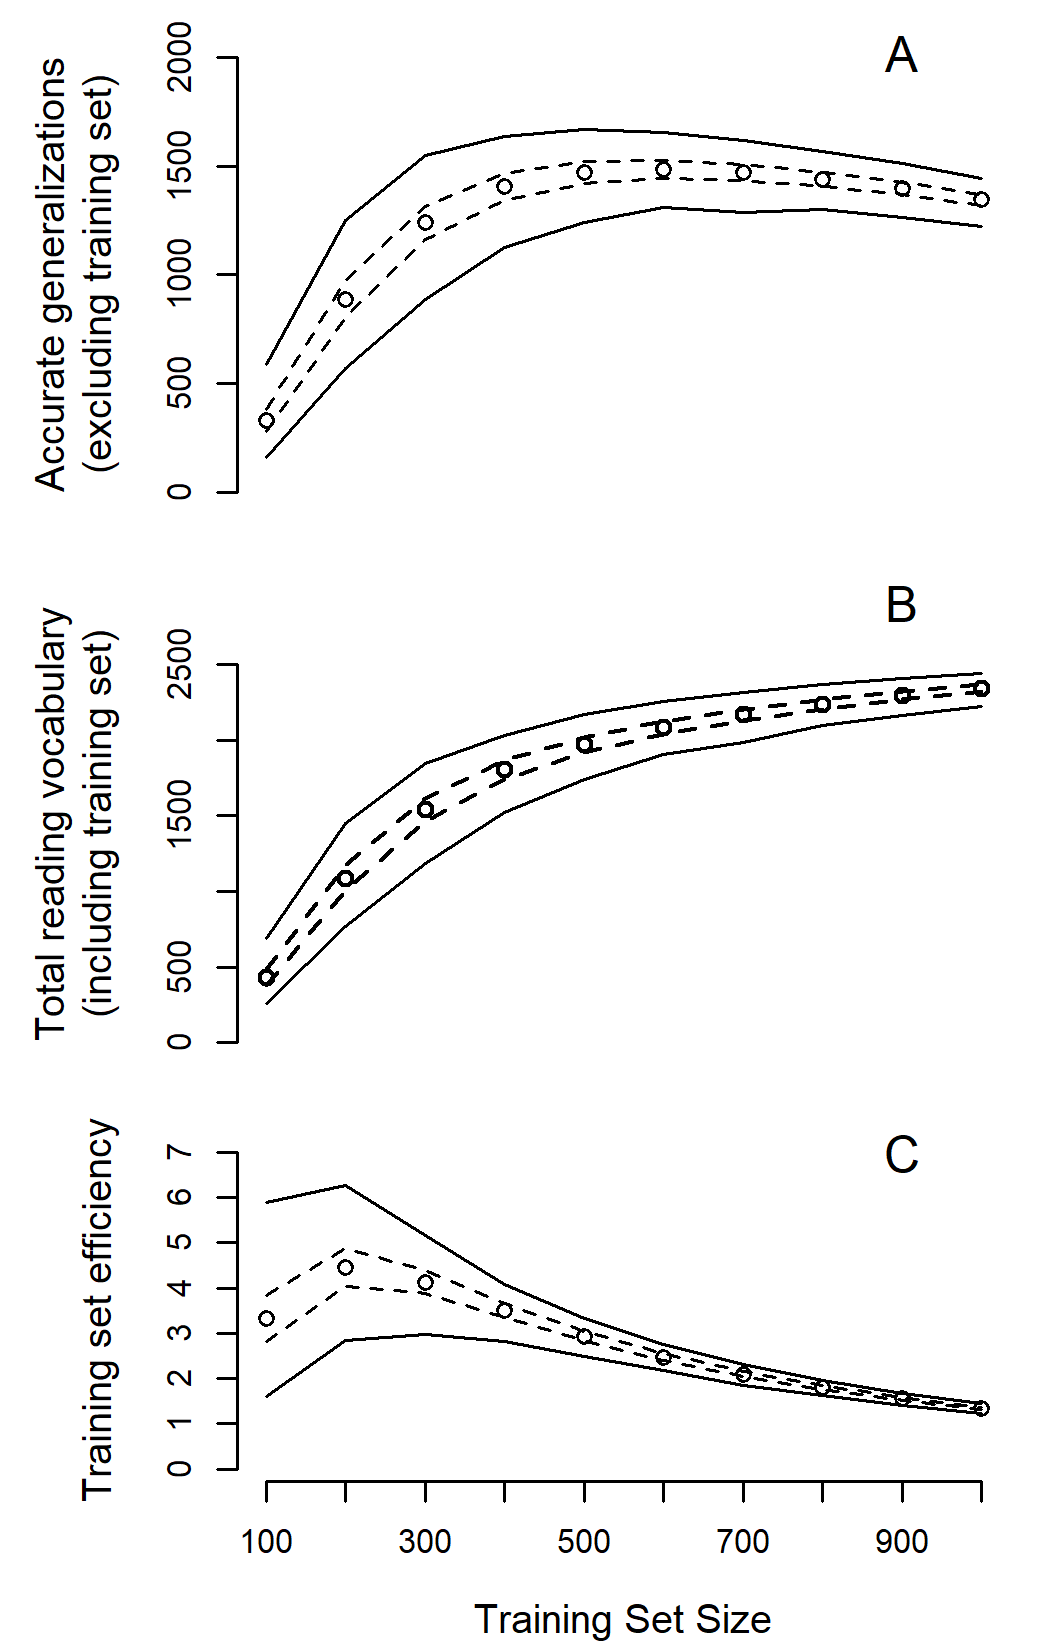
\includegraphics[width=0.9\columnwidth]{figures/generalization_by_setsize.png}

	\caption{Reading vocabulary size and generalization ability for increasing training set sizes. A) The number of accurate generalization peaks at lower training set sizes and B) the rate of reading vocabulary growth slows. No model trained on a subset of words is capable of reading all words. C) The ratio of generalization performance and training set size, efficiency, is highest with training sets with 200--300 words.}
	
	\label{gen_by_setsize}
\end{figure}

Analyses of training environments containing 300 words show that they yielded reading vocabularies of 1540 words on average ($SD = 76.62$) and 1846 words at best (failing to decode 1035). Given that efficiency is a primary concern for early reading curricula, it is noteworthy that this is 75.5\% of the largest reading vocabulary achieved with any training set (2444, achieved after training on 1000 words). Note that this 598 word increase required growing the training set by 700 words. If we subtract the training set from all reading vocabularies and just focus on words that were generalized to, the best model trained on 300 words (1546) achieves 92.7\% of the maximum amount of generalization achieved with any training set (1668, achieved after training on 500 words).

These results indicate that it is possible to establish a reading vocabulary of over 1800 words based on explicit training on only 300 words, a 6 fold return on instructional investment. However, achieving this level of performance is highly dependent on the composition of the training set: the best and worst models trained with 300 words are separated in performance by over 600 accurate generalizations (min: 906; max: 1546). Thus, in future work it will be important to understand how properties of training sets are related to generalization.   

\subsection{What makes a word generalizable?}
There is very high variability in the rate at which individual words are generalized accurately across training contexts, forming a roughly bimodal distribution (Figure \ref{word_acc_hist}).

\begin{figure}[t]
	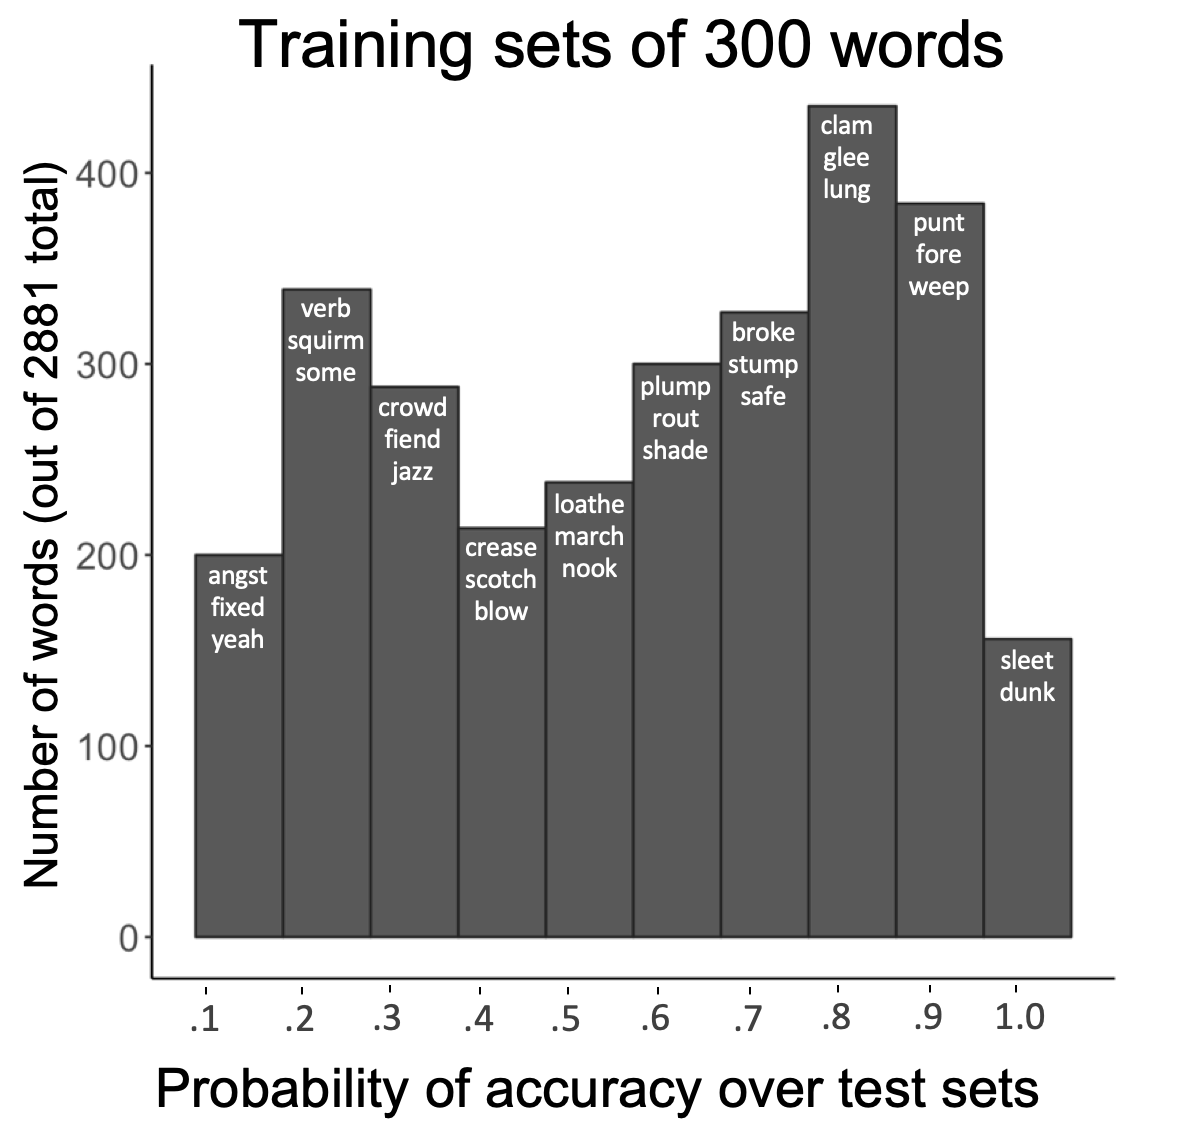
\includegraphics[width=0.9\columnwidth]{figures/word_accuracy_over_testsets.png}

	\caption{When aggregating over the 100k 300-word model training environments, each word occurs in many test sets. The proportion of times a word occurs in the test set and is accurately generalized to corresponds to how difficult that word is to learn. Representative words belonging to each bin are displayed.}
	\label{word_acc_hist}
\end{figure}

At one extreme are words that are accurately generalized to with almost any random selection of words, and at the other are words that can only be accurately generalized to if particular (combinations of) words are present in the training set. This latter set of words has mappings between orthography and phonology that are highly atypical in light of the rest of the corpus, or are comprised of very low frequency combinations of letters, while the former contain spelling patterns and phonological mappings that occur often within the corpus.

Whether a word was likely to be generalized to was related to quantifiable measures of orthographic, phonological, and relational typicality. For each word, we computed the mean pairwise distance between its orthographic representation and the orthographic representations of all other words in the corpus. The same was done for the phonological representations, and representations associated with the mapping between orthography and phonology obtained by training an instance of our model on all words in the corpus until mastery (all phonological outputs are accurate) and extracting the 100 unit hidden layer activation for each word. These will be referred to as the \emph{mapping representations}. Standard deviations (SD) were recorded along with the means of these pairwise distances.

Pairwise average distance in orthographic and phonological space each were correlated with the probability of accurate generalization over words ($r = -0.31$ and $r = -0.28$, respectively). Interestingly, the mean distance among the mapping representations is essentially uncorrelated with accuracy ($r = -0.05$); instead, the SDs associated with these means is the strongest correlate with the probability of accurate generalization ($r = 0.33$). 

The SD of the distances to a point emphasizes its position within the coordinate space in a way that is quite different from the mean. Consider a set of points that fall on a line. If we take one of those points and move it along the line, its mean distance from the other points will change \emph{but the SD of the distances will not}. Now, if we take that same point and pull it off the line, into a second dimension, the mean distance will grow as the point continues its excursion in the new dimension. \emph{The SD among those distances, however, will shrink}. In other words, words with small SDs are likely to occupy idiosyncratic ``representational niches''. We would expect ``sight words'' to occupy such niches, and indeed words like \exword{quay} (pronounced ``key'') and \exword{queue} (pronounced ``cue'') have the lowest SD. Quay in particular has the \nth{2} smallest SD and the \nth{2045} largest mean over distances to the other words; the SD is consistent with its atypicality, while the mean misrepresents it as being very similar to other mappings.

Regressing the probability of accurate generalization for each word on its mean orthographic distance, mean phonological distance, and the SD of distances to mapping representations accounts for 22\% of the overall variance in generalization error, with mapping representation SD metric accounting for 12\% of the variance ($b = 0.23$, $SE = 0.01$, $F(1, 2875) = 383$, $p < 0.001$, $\eta_p^2 = 0.12$, $95\%$, $CI[.25, .21]$). Figure \ref{word_acc_regression} displays model plotted over the accuracy data for each word, with variance explained by orthographic and phonological mean distance removed.

\begin{figure}[t]
	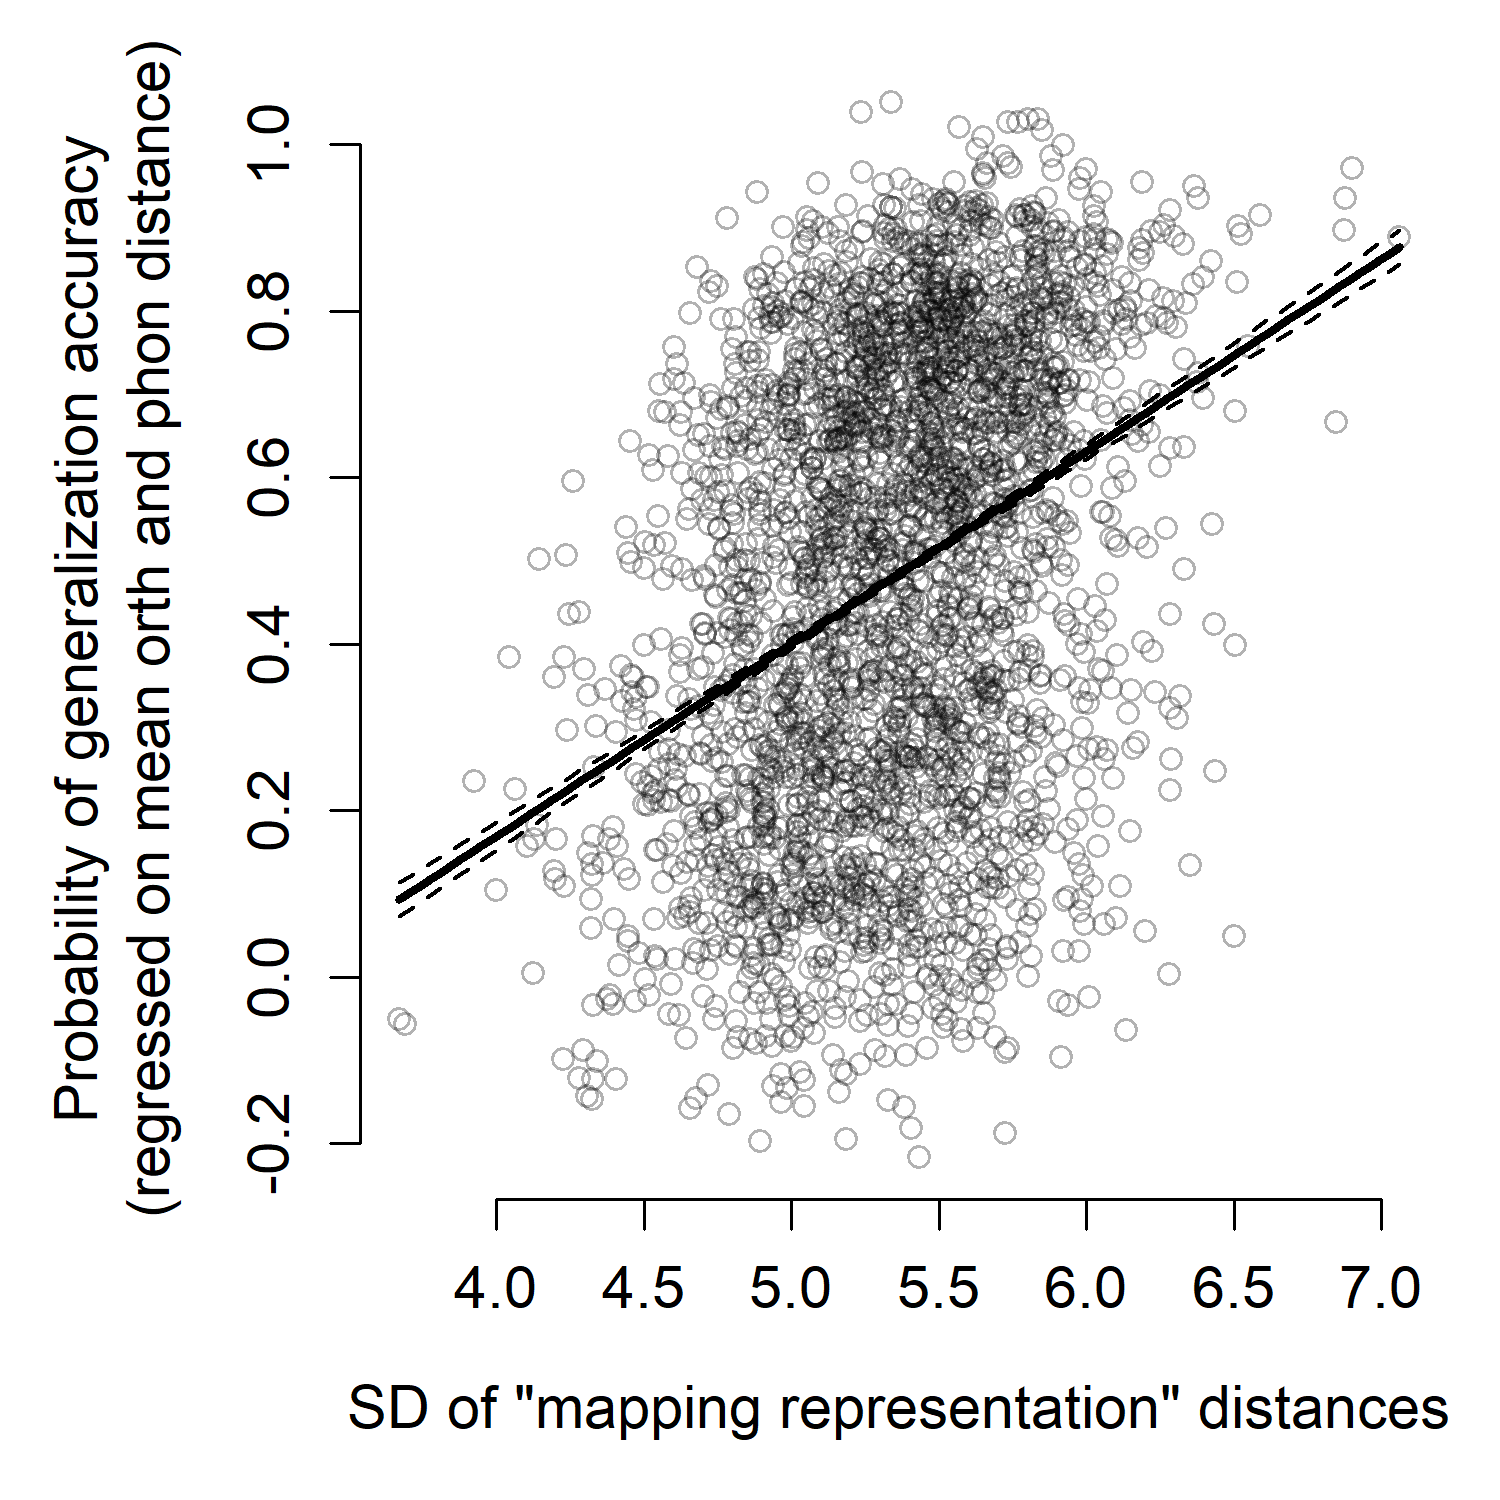
\includegraphics[width=0.9\columnwidth]{figures/word_accuracy_by_hiddenSD.png}

	\caption{The probability of accurate generalization to each word, regressed on the standard deviation (SD) of the distance between each word's ``mapping'' representation and the mapping representations of other words, after removing variance explained by mean orthographic and phonological distance. This metric will be low for words that have a high mean distance while utilizing dimensions in the representational space that are relatively unused by other words.}
	\label{word_acc_regression}
\end{figure}


\subsection{Discussion}
We have established a computational procedure for investigating two aspects of generalization in learning basic reading skills: how many words need to be learned to generalize to real English words yet to be learned, and what aspects of reading vocabulary promote this transfer.  Our findings indicate that while printed vocabulary continues to grow along the number of words taught, the efficiency of learning does not grow along with it.

As the teacher grows the number of words she or he would like to teach, the amount of learning time needed grows along with it. Our findings suggest a trade-off where a smaller number of words could be taught, optimizing efficiency of learning and teaching for sake of near-optimal generalization capacity. This has substantial implications for reading education where very often exhaustive sequential instruction of rule-based mappings from print to sound dominate in pedagogical approaches that consider phonics skills valuable to students.

We don't fully understand the factors of printed vocabulary that promote generalization, both at the word- and set-level. This will be the topic of future research. Follow up simulations will include systematic sampling of words in a theory-driven way with respect to their orth-phon structure, as well as sequencing that input to promote generalization. Nonetheless, these simulations demonstrate that it is possible to be more efficient with curricula that attend to the number of words taught and the words that a prioritized in teaching.


%\section{Acknowledgments}
%The research reported here was supported by the Institute of Education Sciences, US Department of Education, through Award \#R305B150003 to the University of Wisconsin, Madison. The opinions expressed here are those only of the authors and do not at all represent the views of the U.S. Department of Education. The Center for High Throughput Computing (CHTC) is supported by UW-Madison, the Advanced Computing Initiative, the Wisconsin Alumni Research Foundation, the Wisconsin Institutes for Discovery, and the National Science Foundation, and is an active member of the Open Science Grid, which is supported by the National Science Foundation and the U.S. Department of Energy's Office of Science.


\bibliographystyle{apacite}

\setlength{\bibleftmargin}{.125in}
\setlength{\bibindent}{-\bibleftmargin}

\bibliography{CogSci_2019_CoxCooperBorkenhagenSeidenberg}


\end{document}
